% Provenance (never printed): see sources/outline_sources.md (Year 2: ore deposits ---
% magmatic, hydrothermal, sedimentary and supergene deposits; grade and tonnage; exploration).
% Deposit descriptions from the USGS Mineral Deposit Models for Resource Assessment
% (Scientific Investigations Report 2010-5070, chapters A, B, C, E, I, L, N, O, Q), USGS
% Open-File Report 03-077 (orogenic gold) and Grabreck et al. 2022 (kimberlites); the grade and
% tonnage data of the world's porphyry copper deposits from USGS Open-File Report 2008-1155
% (dataset bachelor-2-porphyry-cu). Ledger rows in sources/ledger/book4.md; curves and numbers
% from figdata/bachelor-2/ores.py and the Book 4 second-writer scratch calculator calc/ch29.py.
% Geology and sourced numbers only: no advocacy.
\chapter{Endapan Bijih}\label{ch:b2:ore-deposits}

Tembaga menyusun sekitar \qty{0.006}{\percent} kerak; tembaga ditambang dari batuan yang memuat sekitar
\qty{0.5}{\percent}. Karena itu setiap tambang tembaga terletak di atas batuan yang kira-kira delapan puluh kali lebih kaya daripada
kerak di sekitarnya, dan setiap \omterm{def:b2:ore-deposits:deposit}{endapan bijih} adalah karya suatu pemekat alami: \omterm{def:b2:magma-emplacement:magma}{magma} yang
memisahkan cairan sulfida, air asin panas yang melarutkan logam lalu menjatuhkannya di dalam rekahan, sungai
yang memilah butir berat dari butir ringan, hujan yang melindi bagian atas suatu tubuh bijih dan
mengendapkan kembali tembaganya di bawah. Bab ini mengikuti pemekat-pemekat itu, lalu mengukur
hasilnya --- berapa banyak bijih, dengan kadar berapa --- dan diakhiri dengan cara endapan ditemukan.
% ledger: perkins:ore-grades

\begin{recall}
\textbf{Dari volume-volume sekolah}: \omterm{def:b2:ore-deposits:deposit}{endapan bijih} dan \omterm{def:b2:ore-deposits:cf}{faktor konsentrasi}, urat, \omterm{def:b2:ore-deposits:placer}{plaser}, cadangan, dan
sumber daya; sirkulasi hidrotermal dan perokok hitam di punggung samudra. \textbf{Dari buku-buku
kimia}: bijih; kelarutan, ion kompleks, dan redoks. \textbf{Dari volume Tahun 1}: kecepatan
pengendapan butir dan hukum Stokes; laterit; evaporit. \textbf{Dari
\cref{ch:b2:elements-in-the-earth}}: \omterm{def:b2:elements-in-the-earth:goldschmidt}{unsur kalkofil}, \omterm{def:b2:elements-in-the-earth:partition}{koefisien partisi mineral--lelehan}.
\textbf{Dari \cref{ch:b2:magmatic-differentiation}}: \omterm{def:b2:magmatic-differentiation:cumulate}{intrusi berlapis} dan
\omterm{def:b2:magmatic-differentiation:cumulate}{kumulat}. \textbf{Dari \cref{ch:b2:precambrian-earth}}: \omterm{def:b2:precambrian-earth:bif}{formasi besi berpita}, \omterm{def:b2:precambrian-earth:craton}{kraton}.
\textbf{Dari buku-buku matematika}: distribusi normal dan log-normal, serta fungsi
distribusi normal $\Phi$.
\end{recall}

\section{Bijih, kadar, dan konsentrasi}\label{sec:b2:ore-deposits:grade}

\begin{definition}[Mineral pengotor]\label{def:b2:ore-deposits:ore}
Dalam suatu bijih, yang disebut \emph{mineral pengotor}\index{mineral pengotor} (\textit{gangue}) adalah segala sesuatu yang tidak bernilai ekonomi:
mineral pembentuk batuan, mineral hidrotermal, dan mineral pelapukan yang menyertai mineral bijih lalu
dipisahkan darinya dan dibuang selama pengolahan.
\end{definition}

Sebagian besar bijih adalah \omterm{def:b2:ore-deposits:ore}{mineral pengotor}. Dalam \omterm{def:b2:ore-deposits:hydrothermal}{endapan tembaga porfiri}, sumber utama tembaga dunia, lebih dari
\qty{98}{\percent} bijihnya adalah \omterm{def:b2:ore-deposits:ore}{mineral pengotor}, dan mineral tembaga menyusun sisanya.
% ledger: usgs10b:share

\begin{definition}[Kadar bijih, kadar batas, tonase]\label{def:b2:ore-deposits:grade}
Yang disebut \emph{kadar bijih}\index{kadar bijih} suatu volume batuan adalah fraksi massa unsur atau mineral
berharga di dalamnya: dalam persen untuk logam dasar, dalam gram per ton untuk emas, perak, dan
unsur golongan platina. Yang disebut \emph{kadar batas}\index{kadar batas} adalah kadar terendah
saat suatu blok batuan dihitung sebagai bijih; di bawahnya, blok itu adalah batuan sisa. Yang disebut
\emph{tonase}\index{tonase} suatu endapan adalah massa batuan di atas kadar batas; bersama kadar
rata-ratanya $\bar g$, tonase memberikan logam yang terkandung, $M = T\bar g$.
\end{definition}

Karena itu \omterm{def:b2:ore-deposits:grade}{tonase} dan kadar suatu endapan bukanlah dua fakta tentang batuan, melainkan dua
jawaban atas satu pertanyaan, yang diajukan pada suatu \omterm{def:b2:ore-deposits:grade}{kadar batas} tertentu. Batu Hijau, endapan tembaga--emas porfiri di
Indonesia, dilaporkan sebesar \qty{914}{Mt} dengan \qty{0.53}{\percent} tembaga di atas \omterm{def:b2:ore-deposits:grade}{kadar batas}
\qty{0.3}{\percent}, dan sebesar \qty{1640}{Mt} dengan \qty{0.44}{\percent} dalam suatu kompilasi dunia
yang mengambil \omterm{def:b2:ore-deposits:grade}{kadar batas} terendah yang tersedia: menurunkan \omterm{def:b2:ore-deposits:grade}{kadar batas} hampir menggandakan \omterm{def:b2:ore-deposits:grade}{tonase} dan
menurunkan kadar rata-rata. Dalam suatu endapan seng--timbal sedimenter, endapan Tom di Kanada, penurunan
\omterm{def:b2:ore-deposits:grade}{kadar batas} sekitar satu persen seng ditambah timbal akan melipatlimakan cadangannya.
% ledger: usgs10b:cutoffs, usgs08:tonnage-def, usgs10n:sedex

\begin{definition}[Faktor konsentrasi]\label{def:b2:ore-deposits:cf}
Yang disebut \emph{faktor konsentrasi}\index{faktor konsentrasi} suatu unsur dalam suatu bijih adalah perbandingan
$\mathrm{CF} = g/a$ antara kadarnya $g$ dan kelimpahannya $a$ dalam suatu reservoir acuan, yang disebutkan bersamanya:
seluruh kerak benua, kerak benua atas, atau batuan asal pembentukan endapan itu.
\end{definition}

Faktor itu bergantung pada acuannya. Dengan mengambil \qty{0.006}{\percent} tembaga untuk kerak dan
\qty{0.5}{\percent} untuk bijih diperoleh faktor 83; dengan mengambil kerak benua atas,
\qty{28}{ppm}, dan kadar rata-rata tembaga porfiri pada 2008, \qty{0.44}{\percent}, diperoleh 157. Emas,
dengan \qty{1.5}{ng/g} di kerak atas dan ditambang pada beberapa gram per ton, memiliki faktor dalam
ribuan; besi, dengan beberapa persen di kerak dan ditambang pada sekitar \qty{50}{\percent}, hanya memerlukan
faktor sekitar sepuluh.
% ledger: perkins:ore-grades, rg03:ucc-trace, usgs10b:share, earle:ore-grades, earle:iron-grade

\begin{definition}[Endapan bijih]\label{def:b2:ore-deposits:deposit}
Yang disebut \emph{endapan bijih}\index{endapan bijih} adalah tubuh batuan tempat proses-proses alami telah
memekatkan suatu unsur atau mineral sampai kadar di atas \omterm{def:b2:ore-deposits:grade}{kadar batas}, dengan \omterm{def:b2:ore-deposits:grade}{tonase} yang cukup besar
agar dapat diekstraksi dengan menguntungkan. Endapan bijih sekaligus merupakan objek geologi, yang ditentukan oleh proses-proses yang
membentuknya, dan objek ekonomi, yang ditentukan oleh harga, biaya, dan teknologi.
\end{definition}

Karena separuh ekonominya, ukuran suatu endapan berubah seiring waktu. Sumber daya teridentifikasi suatu unsur
adalah konsentrasi-konsentrasi yang ekstraksinya layak sekarang atau mungkin menjadi layak; cadangannya
adalah bagian yang dapat diekstraksi secara ekonomis pada saat cadangan itu ditentukan. Cadangan tembaga dunia
adalah \qty{280}{Mt} pada 1970; sekitar \qty{697}{Mt} telah ditambang sejak itu, dan cadangan itu
berjumlah \qty{980}{Mt} pada 2024.
% ledger: usgs:mcs-reserves

\begin{proposition}[Neraca massa suatu endapan]\label{prop:b2:ore-deposits:mass-balance}
Suatu endapan yang memuat massa $M$ suatu unsur dengan kadar rata-rata $g$ dipasok oleh sumber yang
kelimpahan unsur itu di dalamnya $a$. Jika proses pemekatan mengekstraksi fraksi $\eta \leq 1$ dari
unsur itu dari sumbernya dan mengantarkannya ke endapan, massa batuan sumber yang diolah adalah
\begin{equation}
m_{\mathrm{source}} = \frac{M}{\eta\,a} = \frac{\mathrm{CF}}{\eta}\, T ,
\label{eq:b2:ore-deposits:mass-balance}
\end{equation}
dengan $T = M/g$ \omterm{def:b2:ore-deposits:grade}{tonase} dan $\mathrm{CF} = g/a$: sedikitnya CF ton sumber per ton bijih.
\end{proposition}

\begin{proof}
Sumber kehilangan $\eta\,a\,m_{\mathrm{source}}$ unsur itu dan endapan menerima $M$; menyamakan
keduanya memberikan bentuk pertama, dan $M = gT$ bentuk kedua. Karena $\eta \leq 1$, $m_{\mathrm{source}} \geq
\mathrm{CF}\,T$.
\end{proof}

Bingham Canyon, endapan porfiri yang ditunjukkan di bawah, tercatat sebesar \qty{3230}{Mt} dengan
\qty{0.882}{\percent} tembaga, yaitu \qty{28.5}{Mt} tembaga. Faktornya terhadap kerak atas adalah 315,
dan bahkan proses yang efisien sempurna harus menguras \num{1.02e12} ton kerak atas
rata-rata, sekitar \qty{377}{km^3}: sebuah kubus bersisi \qty{7.2}{km}. Karena itu proses pembentuk bijih
adalah proses yang memindahkan banyak materi --- \omterm{def:b2:magma-emplacement:magma}{magma}, air, sedimen --- melalui suatu volume
kecil tempat unsur itu terperangkap.
% ledger: data:b4-porphyry-cu, rg03:ucc-trace
% values: 28.49 Mt; CF 315; 1.0175e12 t; 377 km3 at 2.7 t/m3; side 7.22 km (calc/ch29.py)

\begin{omfigure}
\centering
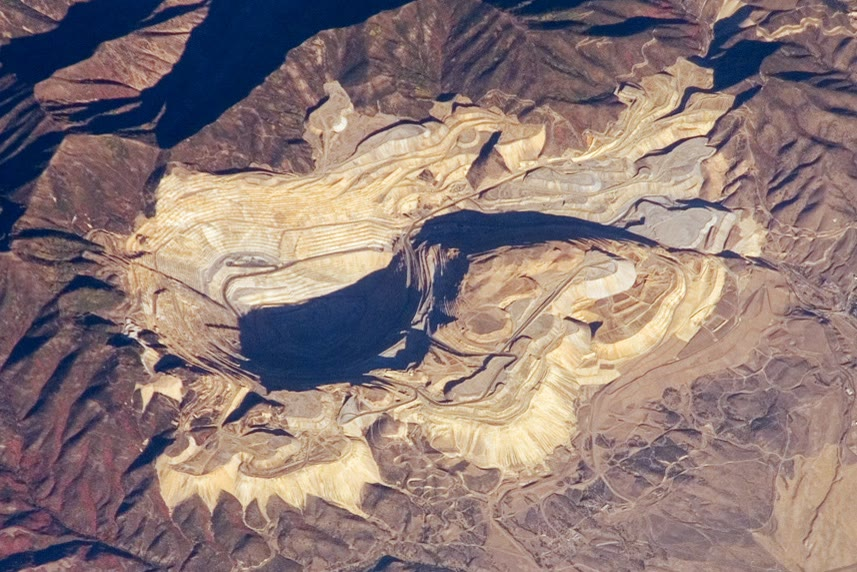
\includegraphics[width=0.5\linewidth]{images/book4/b2-29-bingham-canyon-iss.jpg}
\par\smallskip{\small Tambang terbuka Bingham Canyon, Utah, dari Stasiun Antariksa Internasional
(2007): lebarnya lebih dari \qty{4}{km} dan dalamnya \qty{1200}{m}, dipotong dalam jenjang setinggi 16 sampai \qty{25}{m}
ke dalam suatu \omterm{def:b2:ore-deposits:hydrothermal}{endapan tembaga porfiri}; bukit-bukit berpuncak datar di sekitarnya adalah batuan sisa. (Foto:
NASA, awak Ekspedisi 15, domain publik.)}
\end{omfigure}
% ledger: photo:b2-29-bingham

\begin{definition}[Tipe endapan bijih]\label{def:b2:ore-deposits:types}
Yang disebut \emph{tipe endapan bijih}\index{tipe endapan bijih} adalah kelas endapan yang sama-sama memiliki suatu tatanan
geologi, batuan induk, bentuk, mineralogi bijih, dan proses pembentukan, sehingga deskripsi
kelas itu meramalkan di mana anggota-anggotanya terdapat. Tipe-tipe itu terbagi menjadi empat keluarga menurut prosesnya:
magmatik (logam dipekatkan oleh \omterm{def:b2:magma-emplacement:magma}{magma} ketika mengkristal atau memisah),
hidrotermal (oleh fluida berair yang panas), sedimenter (oleh pengangkutan dan pengendapan
sedimen, atau presipitasi dari air di permukaan), dan supergen (oleh pelapukan
suatu endapan yang lebih awal).
\end{definition}

\section{Endapan magmatik}\label{sec:b2:ore-deposits:magmatic}

\textbf{Kromit dalam \omterm{def:b2:magmatic-differentiation:cumulate}{intrusi berlapis}.} Kromit, satu-satunya sumber kromium komersial,
berkumpul dalam lapisan-lapisan kromitit masif, yang lebih dari \qty{90}{\percent} kromit, di bagian bawah \omterm{def:b2:magmatic-differentiation:cumulate}{intrusi berlapis},
yaitu bagiannya yang ultramafik. Intrusi-intrusi itu berukuran 2 sampai \qty{180}{km} melintang dan tebalnya sampai
\qty{15}{km}, dan lapisannya berkisar dari kurang dari satu sentimeter sampai 5--\qty{8}{m}; bersama-sama
intrusi itu memuat sebagian besar cadangan kromium dunia, dan Kompleks Bushveld, yang telah dijumpai pada
\cref{ch:b2:magmatic-differentiation}, adalah satu-satunya yang kini ditambang untuk kromit. Asal-usulnya, yaitu suatu
lapisan \omterm{def:b2:magmatic-differentiation:cumulate}{kumulat} yang terdorong ke medan kromit oleh percampuran \omterm{def:b2:magma-emplacement:magma}{magma} atau perubahan tekanan atau
keadaan oksidasi, masih diperdebatkan.
% ledger: usgs10e:chromite

\textbf{Sulfida nikel--tembaga--PGE.} \omterm{def:b2:magma-emplacement:magma}{Magma} mafik atau ultramafik, yang dihasilkan oleh derajat pelelehan mantel yang besar
(\qty{20}{\percent} sampai \qty{25}{\percent} atau lebih, dengan lebih dari 12 persen MgO menurut
berat), naik dalam keadaan tak jenuh belerang. Jika \omterm{def:b2:magma-emplacement:magma}{magma} itu mengasimilasi belerang dari kerak, atau mendingin cukup
jauh, \omterm{def:b2:magma-emplacement:magma}{magma} itu menjadi jenuh dan cairan sulfida yang tak bercampur terpisah dalam bentuk butiran-butiran. Logam-logam
kalkofil masuk ke dalam butiran itu: perbandingan $D$ antara konsentrasinya dalam cairan
sulfida dan konsentrasinya dalam cairan silikat, jenis koefisien partisi yang sama dengan yang antara
mineral dan lelehan, adalah $10^2$ sampai $10^3$ untuk tembaga dan nikel serta $10^3$ sampai $10^4$ untuk
unsur golongan platina. Berapa banyak logam yang dikumpulkan suatu butiran lalu bergantung pada berapa banyak \omterm{def:b2:magma-emplacement:magma}{magma} yang dijumpainya.
% ledger: usgs10i:r-factor

\begin{proposition}[Faktor R]\label{prop:b2:ore-deposits:r-factor}
Misalkan satuan massa cairan sulfida terpisah dari, dan mencapai kesetimbangan dengan, massa $R$ \omterm{def:b2:magma-emplacement:magma}{magma}
silikat, yaitu \emph{faktor R}\index{faktor R}, dalam sistem tertutup; misalkan $C_L$ konsentrasi suatu
logam dalam \omterm{def:b2:magma-emplacement:magma}{magma} sebelum sulfida terpisah, dan $D$ koefisien partisi sulfida--silikatnya.
Maka konsentrasi logam itu dalam sulfida adalah
\begin{equation}
C_S = C_L\,\frac{D\,(R + 1)}{R + D} .
\label{eq:b2:ore-deposits:r-factor}
\end{equation}
Untuk $R \gg D$, $C_S \to D\,C_L$; untuk $R \ll D$, $C_S \approx (R + 1)\,C_L$.
\end{proposition}

\begin{proof}
Sistem bermassa $R + 1$ memuat $(R + 1)C_L$ logam itu sebelum pemisahan. Setelahnya, silikat
memuat $R\,C_{\mathrm{sil}}$ dan sulfida $C_S$, dengan $C_S = D\,C_{\mathrm{sil}}$ pada kesetimbangan.
Kekekalan memberikan $(R + 1)C_L = R\,C_S/D + C_S = C_S\,(R + D)/D$, sehingga diperoleh
\eqref{eq:b2:ore-deposits:r-factor}. Jika $R \gg D$, $(R + 1)/(R + D) \to 1$; jika $R \ll D$,
$D/(R + D) \to 1$.
\end{proof}

Kedua limit itu menjelaskan mengapa ada dua jenis bijih sulfida. Bila $R \ll D$, sulfida mengambil
hampir semua logam \omterm{def:b2:magma-emplacement:magma}{magma} yang dijumpainya dan $C_S$ tumbuh seiring $R$; bila $R \gg D$, sulfida itu
jenuh pada $D\,C_L$ dan tambahan \omterm{def:b2:magma-emplacement:magma}{magma} tidak menambahkan apa pun. Nikel dan tembaga, dengan $D$ beberapa ratus,
mencapai batas atasnya pada $R$ beberapa ratus sampai beberapa ribu, rentang kebanyakan bijih nikel--tembaga;
platina dan paladium, dengan $D$ dekat $10^4$, terus bertambah sampai $R$ sebesar \num{10000} sampai
\num{100000}. Karena itu bijih yang kaya akan unsur golongan platina, seperti Merensky Reef di Bushveld dan
sebagian bijih Noril'sk, merekam massa sulfida yang kecil yang dibilas oleh massa \omterm{def:b2:magma-emplacement:magma}{magma} yang sangat
besar (latihan~\ref{exo:b2:ore-deposits:5} dan~\ref{exo:b2:ore-deposits:11}).
% ledger: usgs10i:r-factor

\textbf{Kimberlit dan intan.} Kebanyakan intan, dan hampir semua intan yang ditambang, terbentuk di dasar
litosfer benua yang tebal, di akar \omterm{def:b2:precambrian-earth:craton}{kraton}; \omterm{def:b2:magma-emplacement:magma}{magma} kimberlit, yang berasal dari kedalaman
lebih dari 120 sampai \qty{150}{km} dan naik dengan kecepatan sampai \qty{20}{m.s^{-1}}, membawanya ke
permukaan cukup cepat sehingga intan itu bertahan. Kimberlit lebih suka meletus melalui litosfer yang tebal dan tua,
dan di situlah eksplorasi intan mencari.
% ledger: grabreck22:kimberlite

\textbf{Pegmatit.} Pegmatit litium--sesium--tantalum adalah \omterm{def:b2:magma-emplacement:bodies}{retas} granitik yang diperkaya dengan unsur-unsur
langka ini, yang dihasilkan di \omterm{def:b2:himalaya-andes:types}{orogen tumbukan}; pegmatit itu mengkristal pada sekitar 350 sampai \qty{550}{\celsius},
sangat rendah untuk lelehan granitik, dalam beberapa hari sampai beberapa tahun, dan menumbuhkan kristal yang sangat besar --- satu
kristal spodumen panjangnya \qty{14}{m}. Mineral litiumnya, yaitu spodumen, petalit, dan
lepidolit, memasok sekitar seperempat litium dunia.
% ledger: usgs10o:lct

\section{Endapan hidrotermal}\label{sec:b2:ore-deposits:hydrothermal}

\begin{definition}[Fluida hidrotermal dan tipe-tipe endapan hidrotermal]\label{def:b2:ore-deposits:hydrothermal}
Yang disebut \emph{fluida hidrotermal}\index{fluida hidrotermal} adalah fluida berair yang panas, yang dilepaskan oleh \omterm{def:b2:magma-emplacement:magma}{magma},
oleh \omterm{def:b2:metamorphic-facies:reaction}{reaksi metamorfik}, atau berupa air laut, air meteorik, atau air asin cekungan yang terpanaskan, yang melarutkan,
mengangkut, dan mengendapkan unsur-unsur ketika mengalir melalui batuan. \omterm{def:b2:ore-deposits:types}{Tipe endapan bijih} hidrotermal yang utama
adalah:
\begin{itemize}
  \item \emph{endapan tembaga porfiri}\index{endapan tembaga porfiri}: tubuh besar berkadar rendah
        yang terdiri atas urat-urat halus dan sulfida tembaga tersebar di dalam dan di sekitar stok porfiri yang kecil, yang terbentuk oleh
        fluida magmatik dalam beberapa kilometer dari permukaan di atas zona subduksi;
  \item \emph{endapan epitermal}\index{endapan epitermal}: urat dan sebaran emas--perak
        yang terbentuk dalam sekitar \qty{1.5}{km} dari permukaan, pada sekitar 100 sampai
        \qty{300}{\celsius}, di busur vulkanik;
  \item \emph{endapan sulfida masif vulkanogenik}\index{endapan sulfida masif vulkanogenik}
        (VMS): lensa sulfida masif yang terbentuk di atas atau tepat di bawah dasar laut, pada lubang
        hidrotermal dalam tatanan vulkanik bawah laut;
  \item \emph{endapan ekshalatif sedimen}\index{endapan ekshalatif sedimen} (sedex):
        sulfida seng--timbal berlapis tipis di dalam serpih laut suatu \omterm{def:b2:basins-compared:types}{cekungan celah}, yang terendapkan di atas atau tepat
        di bawah dasar laut dari air asin cekungan yang naik di sepanjang sesar;
  \item \emph{endapan tipe Mississippi Valley}\index{endapan tipe Mississippi Valley} (MVT):
        sulfida seng--timbal yang menggantikan karbonat paparan, epigenetik dan tidak berkaitan dengan aktivitas
        beku, yang diendapkan oleh air asin cekungan;
  \item \emph{endapan emas orogenik}\index{endapan emas orogenik}: urat kuarsa pembawa emas di
        sabuk metamorfik, di sepanjang sesar-sesar besar, yang diendapkan oleh fluida bersalinitas rendah dan kaya CO$_2$ yang
        berasal dari \omterm{def:b2:metamorphic-facies:metamorphism}{metamorfisme}.
\end{itemize}
\end{definition}
% ledger: usgs10b:form, usgs10q:epithermal, usgs10c:vms, usgs10n:sedex, usgs10a:mvt, drew03:orogenic

\textbf{Pengangkutan dan pengendapan.} Kebanyakan logam diangkut dalam \omterm{def:b2:ore-deposits:hydrothermal}{fluida hidrotermal} sebagai kompleks:
seng, timbal, dan tembaga sebagai kompleks klorida, sehingga salinitas mengendalikan kelarutannya, dan emas,
dalam fluida tereduksi, sebagai kompleks belerang seperti AuHS(H$_2$S)$_3$. Suatu fluida menjatuhkan muatannya ketika
kelarutannya turun: ketika mendingin; ketika mendidih karena tekanannya turun, sehingga kehilangan H$_2$S dan CO$_2$ dan
pH-nya berubah; ketika bercampur dengan fluida berkomposisi lain --- air asin yang bertemu air kaya
H$_2$S mengendapkan sfalerit dan galena hampir seketika; dan ketika bereaksi dengan batuan
dinding, yang mengubah pH atau keadaan oksidasinya. Setiap tipe endapan adalah satu kombinasi fluida,
lintasan, dan perangkap.
% ledger: usgs10n:sedex, drew03:orogenic

\textbf{Tembaga porfiri.} Endapan porfiri memasok sekitar \qty{60}{\percent} tembaga dunia
dan memuat sekitar \qty{65}{\percent} sumber dayanya. Endapan itu berpusat pada stok-stok silindris yang kecil
atau kawanan \omterm{def:b2:magma-emplacement:bodies}{retas}, puncak-puncak \omterm{def:b2:magma-emplacement:bodies}{pluton} yang lebih besar, yang ditempatkan pada kedalaman kurang dari 5--\qty{10}{km} di
busur di atas zona subduksi, tatanan pada \cref{ch:b2:magmatic-series}. Suatu endapan berukuran 0.1 sampai
\qty{1}{km} melintang, dengan tinggi yang serupa; batuan teralterasi dapat meluas \qty{10}{km} atau lebih di sekitarnya.
Ketika \omterm{def:b2:magma-emplacement:magma}{magma} mengkristal, fluida dengan 3 sampai 5 persen garam menurut berat terpisah darinya; ketika naik dan
mengalami dekompresi, fluida itu terbelah menjadi air asin dan uap, keduanya membawa logam, dan tekanan berlebihnya
meretakkan batuan. Urat kuarsa terendapkan pada sekitar 700 sampai \qty{500}{\celsius}, dan
reaksi fluida dengan batuan menzonakan alterasinya, seperti pada penampang di bawah. Karena
endapan ini terbentuk dangkal di tepi aktif, tempat erosi berlangsung cepat, lebih dari \qty{90}{\percent} endapan porfiri
yang diketahui berumur Kenozoikum atau Mesozoikum.
% ledger: usgs10b:share, usgs10b:form, usgs10b:fluids, usgs10b:alteration

\begin{omfigure}
\centering
\begin{tikzpicture}[x=1.15cm, y=1.15cm, font=\small]
\begin{scope}
\clip (-2.9,-3.6) rectangle (2.9,0);
% propylitic halo
\fill[omLithBasalt!45] (0,-1.25) ellipse (2.45 and 1.55);
% sodic-calcic deep flanks
\fill[omExo!25] (-1.75,-2.55) ellipse (0.45 and 0.38);
\fill[omExo!25] (1.75,-2.55) ellipse (0.45 and 0.38);
% sericitic shell
\fill[yellow!35] (0,-1.05) ellipse (1.15 and 1.15);
% potassic core
\fill[omProp!40] (0,-1.45) ellipse (0.68 and 0.85);
% ore shell
\draw[omThm, line width=1.1pt, densely dashed] (0,-1.3) ellipse (0.92 and 0.98);
% advanced argillic lithocap
\fill[omDef!30] (-1.05,0) .. controls (-0.6,-0.5) and (0.6,-0.5) .. (1.05,0) -- cycle;
\draw[omDef!70] (-1.05,0) .. controls (-0.6,-0.5) and (0.6,-0.5) .. (1.05,0);
\end{scope}
% pluton and stock
\fill[omLithGranite] (-2.6,-3.6) .. controls (-2.2,-2.9) and (-0.9,-2.6) .. (-0.3,-2.6)
  -- (-0.3,-1.25) arc[start angle=180, end angle=0, radius=0.3] -- (0.3,-2.6)
  .. controls (0.9,-2.6) and (2.2,-2.9) .. (2.6,-3.6) -- cycle;
\draw[black!60] (-2.6,-3.6) .. controls (-2.2,-2.9) and (-0.9,-2.6) .. (-0.3,-2.6)
  -- (-0.3,-1.25) arc[start angle=180, end angle=0, radius=0.3] -- (0.3,-2.6)
  .. controls (0.9,-2.6) and (2.2,-2.9) .. (2.6,-3.6);
% epithermal veins
\foreach \x in {1.45,1.65,1.85} \draw[omDef, line width=1pt] (\x,-0.02) -- (\x+0.12,-0.7);
% palaeosurface
\draw[black, line width=0.8pt] (-2.9,0) -- (2.9,0);
\node[anchor=south west, font=\scriptsize] at (-2.9,0) {paleopermukaan};
% labels
\draw[black!50] (0.6,-0.15) -- (1.2,0.25) -- (3.0,0.25) node[anchor=west, text=black] {argilik lanjut};
\draw[black!50] (1.95,-0.3) -- (3.0,-0.3) node[anchor=west, text=black] {urat epitermal};
\draw[black!50] (1.05,-0.8) -- (3.0,-0.8) node[anchor=west, text=black] {serisitik};
\draw[black!50] (0.85,-1.25) -- (3.0,-1.25) node[anchor=west, text=omThm] {cangkang bijih tembaga};
\draw[black!50] (0.45,-1.7) -- (3.0,-1.7) node[anchor=west, text=black] {potasik};
\draw[black!50] (1.05,-2.15) -- (3.0,-2.15) node[anchor=west, text=black] {propilitik};
\draw[black!50] (2.1,-2.6) -- (3.0,-2.6) node[anchor=west, text=black] {sodik--kalsik};
\draw[black!50] (1.5,-3.15) -- (3.0,-3.15) node[anchor=west, text=black] {pluton dan stok porfiri};
\end{tikzpicture}
\par\smallskip{\small Suatu sistem tembaga porfiri dalam penampang (gambar, tidak berskala): zona
potasik di inti, dalam dan panas; zona serisitik ke atas dan ke luar, tempat pirit
melimpah; cangkang bijih tembaga di antara keduanya; halo propilitik pada kedalaman dangkal sampai sedang
di sekelilingnya; alterasi sodik--kalsik di sayap-sayap yang dalam; tudung argilik lanjut dan, pada sebagian
sistem, urat epitermal di dekat permukaan.}
\end{omfigure}
% ledger: usgs10b:alteration

\textbf{Emas epitermal.} Di atas sebagian sistem porfiri, dan di busur vulkanik pada umumnya, fluida yang
sejenis mencapai \qty{1.5}{km} teratas kerak pada sekitar 100 sampai \qty{300}{\celsius},
tempat fluida itu mendidih dan bercampur dengan air tanah; fluida itu mengendapkan emas dan perak dalam urat kuarsa, dengan
alterasi yang merekam fluida yang hampir netral (adularia, ilit) atau yang sangat asam (kaolinit,
dikit, pirofilit).
% ledger: usgs10q:epithermal, usgs10q:alteration

\textbf{Sulfida masif di dasar laut.} Air laut yang tertarik turun ke dalam kerak panas suatu punggung samudra atau
busur kembali melalui lubang-lubang sebagai perokok hitam pada sekitar \qty{350}{\celsius}, yang pertama kali terlihat di Punggung
Pasifik Timur pada 1979. Di tempat lapangan lubang itu bertahan lama, sulfidanya membangun suatu gundukan; bijihnya lebih dari
\qty{40}{\percent} sulfida, di atas jaringan urat (\textit{stockwork}) yang menandai saluran pengumpannya. Logam-logamnya terzonasi
menurut suhu, besi dan tembaga di dasar yang panas, seng, besi, timbal, dan barium di bagian atas dan
tepi yang lebih dingin, seperti pada gundukan yang digambar pada subbab berikutnya. \omterm{def:b2:ore-deposits:hydrothermal}{Endapan sulfida masif
vulkanogenik} berkisar dari kantong yang kurang dari satu ton sampai \qty{1.5}{Gt} Rio Tinto di Spanyol, dan
umurnya dari \qty{3.55}{\Ga} sampai endapan yang terbentuk saat ini.
% ledger: usgs10c:vms

\textbf{Air asin cekungan: sedex dan MVT.} Air asin cekungan dengan 10 sampai \qty{30}{\percent} garam terlarut,
yang terpanaskan sampai 100--\qty{200}{\celsius} oleh penimbunan, membawa seng dan timbal sebagai kompleks klorida dan membentuk
kedua tipe yang berinduk sedimen. Endapan sedex terbentuk di tempat air asin itu keluar ke dalam cekungan yang terbatas dan tereduksi
di sepanjang sesar celah dan bertemu hidrogen sulfida, sehingga membentuk lumpur sulfida berlapis tipis; endapan ini memuat lebih
dari separuh cadangan seng dan timbal dunia. Endapan MVT terbentuk di tempat air asin, yang terdorong keluar dari suatu
cekungan, mencapai paparan karbonat di tepinya dan menggantikannya pada 75 sampai sekitar
\qty{200}{\celsius}; endapan ini memuat \qty{38}{\percent} timbal dan seng dari endapan yang berinduk sedimen,
dengan seng kira-kira sepuluh kali lebih banyak daripada timbal.
% ledger: usgs10n:sedex, usgs10a:mvt

\textbf{Emas orogenik.} Di sabuk metamorfik, reaksi-reaksi devolatilisasi melepaskan fluida yang hampir netral,
bersalinitas rendah, dan kaya CO$_2$; fluida itu, yang disalurkan di sepanjang sesar-sesar besar, mengendapkan urat kuarsa
pembawa emas pada sekitar \qty{350}{\celsius} dan kedalaman 4 sampai \qty{12}{km}. Urat-urat itu menerus sepanjang
ketinggian yang besar: \qty{3.2}{km} di Kolar, India.
% ledger: drew03:orogenic

\section{Endapan sedimenter dan supergen}\label{sec:b2:ore-deposits:sedimentary}

\begin{definition}[Plaser]\label{def:b2:ore-deposits:placer}
Yang disebut \emph{plaser}\index{plaser} adalah endapan sedimenter berupa mineral yang padat dan tahan lama, yang dipekatkan oleh
air atau angin yang bergerak karena, untuk ukuran yang sama, mineral itu mengendap lebih cepat dan kurang mudah terangkut
daripada butir-butir kuarsa di sekitarnya.
\end{definition}

Mineral yang lebih padat daripada sekitar 2.85 disebut mineral berat, dibandingkan dengan 2.65 untuk kuarsa: ilmenit dan zirkon
dekat 4.7, magnetit 5.2, emas 15 sampai 19.3. Menurut hukum Stokes kecepatan pengendapan suatu butir tumbuh seiring
kelebihan densitasnya $\rho_s - \rho_w$, sebelas kali lebih besar untuk emas daripada untuk kuarsa, sehingga emas dengan
ukuran tertentu berada bersama kuarsa yang tiga kali lebih besar (latihan~\ref{exo:b2:ore-deposits:3}); emas
biasanya tetap berada dalam kerikil sungai di atas batuan dasar, sedangkan ilmenit, rutil, dan zirkon mencapai pantai dan
gumuk. Kadar dalam pasir mineral berat adalah persen berat mineral berat.
% ledger: usgs10l:heavy, usgs:gold-placer

Sedimen kimia juga merupakan bijih. \omterm{def:b2:precambrian-earth:bif}{Formasi besi berpita} pada \cref{ch:b2:precambrian-earth},
yang terendapkan ketika besi terlarut samudra teroksidasi, adalah bijih besi yang umum; evaporit
memasok halit dan garam kalium; laterit, sisa pelapukan tropis yang dalam,
memekatkan aluminium sebagai bauksit. Pelapukan juga meningkatkan kadar endapan-endapan yang lebih awal.
% ledger: earle:bif, usgs:bauxite

\begin{definition}[Pengayaan supergen, gossan]\label{def:b2:ore-deposits:supergene}
Yang disebut \emph{pengayaan supergen}\index{pengayaan supergen} adalah pemekatan suatu logam oleh
air tanah yang turun: di atas muka air tanah, air asam yang beroksigen melarutkan logam dari
sulfida suatu tubuh bijih, dan di bawahnya, dalam kondisi reduksi, mengendapkannya kembali, terutama dengan
menggantikan sulfida primer. Yang disebut \emph{gossan}\index{gossan} adalah batuan berpori yang kaya oksida besi, yang
tertinggal di permukaan di atas tubuh sulfida yang lapuk, dengan sulfidanya digantikan oleh goetit, hematit, dan
jarosit.
\end{definition}

Pada endapan porfiri, tudung terlindi di atas muka air tanah tebalnya sampai beberapa ratus meter;
di bawahnya, zona sulfida yang diperkaya berupa kalkosit, setebal puluhan sampai beberapa ratus meter, mencapai
lebih dari \qty{1.5}{Gt} dengan 0.4 sampai \qty{1.7}{\percent} tembaga, selalu lebih kaya daripada bijih primer
hipogen di bawahnya. Oksida besi suatu \omterm{def:b2:ore-deposits:supergene}{gossan} dan suatu tudung terlindi mempertahankan tekstur
sulfida yang digantikannya, dan menjadi petunjuk pencarian di bawahnya; \omterm{def:b2:ore-deposits:supergene}{gossan} dan noda besinya mengungkapkan banyak
endapan sulfida masif kepada para penambang awal.
% ledger: usgs10b:supergene, usgs10c:vms

\begin{omfigure}
\centering
\begin{minipage}[b]{0.46\linewidth}\centering
\begin{tikzpicture}[x=1cm, y=1cm, font=\scriptsize]
\fill[omHist!55] (0,4.0) rectangle (1.8,5.2);
\fill[omMeth!30] (0,3.0) rectangle (1.8,4.0);
\fill[black!55] (0,1.8) rectangle (1.8,3.0);
\fill[black!18] (0,0) rectangle (1.8,1.8);
\draw (0,0) rectangle (1.8,5.2);
\draw[omDef, line width=1pt, densely dashed] (-0.25,3.0) -- (2.05,3.0);
\foreach \x in {0.45,0.9,1.35} \draw[omDef, -{Stealth[length=4pt]}] (\x,5.0) -- (\x,3.2);
\node[anchor=west, align=left] at (2.0,4.6) {gossan dan tudung\\terlindi (oksida Fe)};
\node[anchor=west, align=left] at (2.0,3.5) {zona oksida\\(malakit)};
\node[anchor=east, text=omDef, align=right] at (-0.25,3.0) {muka\\air tanah};
\node[anchor=west, align=left] at (2.0,2.4) {selimut pengayaan\\(kalkosit)};
\node[anchor=west, align=left] at (2.0,0.9) {bijih primer\\(kalkopirit\\+ pirit)};
\node[anchor=south, font=\scriptsize, text=omDef] at (0.9,5.25) {air asam, Cu$^{2+}$};
\end{tikzpicture}
\end{minipage}\hfill
\begin{minipage}[b]{0.52\linewidth}\centering
\begin{tikzpicture}[x=1cm, y=1cm, font=\scriptsize]
\fill[omSea] (-2.6,1.4) rectangle (2.6,3.2);
\fill[omLithBasalt!60] (-2.6,-1.6) rectangle (2.6,1.4);
% stockwork cone
\fill[omProp!25] (-0.5,-1.6) -- (0.5,-1.6) -- (1.1,0.9) -- (-1.1,0.9) -- cycle;
\foreach \x/\y in {-0.3/-1.2,0.1/-1.0,-0.6/-0.4,0.4/-0.3,-0.1/0.1,0.6/0.4,-0.7/0.5}
  \draw[omProp!80!black] (\x,\y) -- ++(0.35,0.25);
% mound: upper rim and core
\fill[yellow!45] (-1.8,1.4) .. controls (-1.2,2.35) and (1.2,2.35) .. (1.8,1.4) -- cycle;
\fill[omThm!45] (-1.1,1.4) .. controls (-0.7,2.0) and (0.7,2.0) .. (1.1,1.4) -- cycle;
\draw (-1.8,1.4) .. controls (-1.2,2.35) and (1.2,2.35) .. (1.8,1.4);
% chimney and plume
\fill[black!70] (-0.08,2.1) rectangle (0.08,2.55);
\fill[black!45] (0,2.6) circle (0.12) (0.1,2.8) circle (0.16) (0.25,3.0) circle (0.2);
\draw[omDef, -{Stealth[length=4pt]}] (-2.3,2.9) -- (-2.3,0.2) -- (-1.2,-0.9);
\draw[omThm, -{Stealth[length=4pt]}] (0,-1.5) -- (0,1.2);
\node[anchor=west, text=omDef] at (-2.55,3.05) {air laut};
\node[anchor=west] at (0.45,2.85) {perokok hitam, \qty{350}{\celsius}};
\draw[black!50] (1.45,1.75) -- (2.0,2.15) node[anchor=west, text=black] {Zn, Fe, Pb, Ba};
\draw[black!50] (0.6,1.6) -- (2.0,1.15) node[anchor=west, text=black] {Fe, Cu};
\node[anchor=west, align=left] at (0.95,-0.4) {jaringan urat\\(pengumpan)};
\node[anchor=north, text=omThm] at (0,-1.6) {fluida panas};
\end{tikzpicture}
\end{minipage}
\par\smallskip{\small Kiri: profil supergen di atas tubuh sulfida tembaga (gambar, tidak
berskala): air asam melindi tembaga di atas muka air tanah dan mengendapkannya kembali sebagai kalkosit di bawahnya,
dengan meninggalkan \omterm{def:b2:ore-deposits:supergene}{gossan} di permukaan. Kanan: gundukan sulfida masif vulkanogenik dalam penampang (suatu
gambar): air laut yang terpanaskan di dalam kerak naik melalui jaringan urat dan keluar sebagai perokok hitam;
gundukan itu terzonasi dari besi dan tembaga di dasar yang panas sampai seng, besi, timbal, dan barium di bagian atas dan
tepinya.}
\end{omfigure}
% ledger: usgs10b:supergene, usgs10c:vms

\begin{omfigure}
\centering
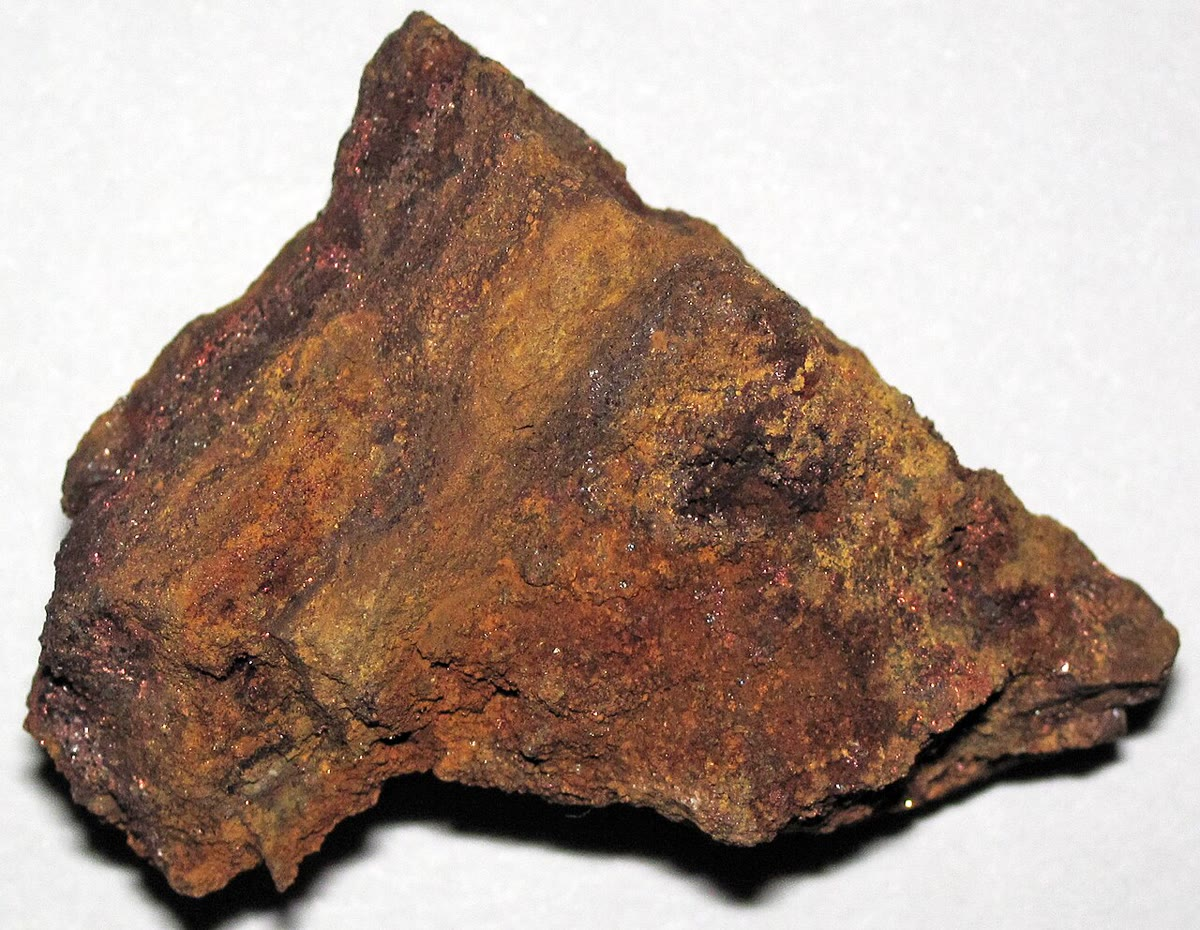
\includegraphics[width=0.4\linewidth]{images/book4/b2-29-flambeau-gossan.jpg}
\par\smallskip{\small \omterm{def:b2:ore-deposits:supergene}{Gossan} dari endapan sulfida masif Flambeau, Wisconsin: batuan berpori dari
hidroksi-oksida besi yang tertinggal oleh pelapukan pirit, kalkopirit, kalkosit, dan bornit dalam suatu
busur vulkanik Paleoproterozoikum; bintik-bintik kecil berwarna jingga adalah tembaga nativ. (Foto: James St.
John, CC~BY~2.0.)}
\end{omfigure}
% ledger: photo:b2-29-gossan

\section{Kadar dan tonase}\label{sec:b2:ore-deposits:grade-tonnage}

Suatu kompilasi dunia mendaftar 422 \omterm{def:b2:ore-deposits:hydrothermal}{endapan tembaga porfiri} beserta \omterm{def:b2:ore-deposits:grade}{tonasenya}, pada \omterm{def:b2:ore-deposits:grade}{kadar batas} terendah
yang tersedia, dan kadar tembaga rata-ratanya. Sepersepuluh di antaranya melebihi \qty{1500}{Mt} dan sepersepuluh memuat kurang
dari \qty{33}{Mt}, dengan median \qty{240}{Mt}; kadarnya berkisar dari \qty{0.24}{\percent} sampai
\qty{0.75}{\percent} di antara desil-desil yang sama, dengan median \qty{0.44}{\percent}. Di antara
desil-desil itu \omterm{def:b2:ore-deposits:grade}{tonase} tersebar dalam faktor 45, sedangkan kadar dalam faktor 3. Pada sumbu logaritmik kedua histogram dekat dengan kurva normal, seperti yang ditunjukkan gambar di bawah:
logaritma \omterm{def:b2:ore-deposits:grade}{tonase} memiliki rata-rata 2.373 dan simpangan baku 0.654, sedangkan logaritma kadar
$-0.364$ dan 0.199 (logaritma berbasis 10, \omterm{def:b2:ore-deposits:grade}{tonase} dalam megaton, kadar dalam persen). Kecocokannya
tidak sempurna: kadar-kadar itu lebih runcing daripada hukum log-normal, dan beberapa endapan berkadar sangat rendah membuat
kadar menyimpang dari hukum itu dalam uji formal. Lagi pula keduanya hampir saling bebas, dengan korelasi
0.1 di antara logaritmanya.
% ledger: usgs08:table1, usgs08:independence, data:b4-porphyry-cu

\begin{omfigure}
\centering
\begin{minipage}[b]{0.49\linewidth}\centering
\begin{tikzpicture}
\begin{axis}[omrecord, width=0.96\linewidth, height=4.5cm, xmin=0.5, xmax=5.0, ymin=0, ymax=80,
  xlabel={tonase (Mt)}, ylabel={jumlah endapan},
  xtick={1,2,3,4,5}, xticklabels={10,100,1000,$10^4$,$10^5$},
  tick label style={font=\scriptsize}, label style={font=\small}]
% computed in figdata/bachelor-2/ores.py part hist_t; ledger: data:b4-porphyry-cu
\addplot[ybar, bar width=0.22, fill=omDef!35, draw=omDef!70] table[x=log10_t, y=count] {figdata/out/bachelor-2-ores-hist_t.dat};
\addplot[omThm, line width=1pt, smooth] table[x=log10_t, y=fit] {figdata/out/bachelor-2-ores-hist_t.dat};
\end{axis}
\end{tikzpicture}
\end{minipage}\hfill
\begin{minipage}[b]{0.49\linewidth}\centering
\begin{tikzpicture}
\begin{axis}[omrecord, width=0.96\linewidth, height=4.5cm, xmin=-1.2, xmax=0.6, ymin=0, ymax=120,
  xlabel={kadar tembaga (\%)}, ylabel={jumlah endapan},
  xtick={-1,-0.69897,-0.30103,0,0.30103}, xticklabels={0.1,0.2,0.5,1,2},
  tick label style={font=\scriptsize}, label style={font=\small}]
% computed in figdata/bachelor-2/ores.py part hist_g; ledger: data:b4-porphyry-cu
\addplot[ybar, bar width=0.088, fill=omDef!35, draw=omDef!70] table[x=log10_g, y=count] {figdata/out/bachelor-2-ores-hist_g.dat};
\addplot[omThm, line width=1pt, smooth] table[x=log10_g, y=fit] {figdata/out/bachelor-2-ores-hist_g.dat};
\end{axis}
\end{tikzpicture}
\end{minipage}
\par\smallskip{\small \omterm{def:b2:ore-deposits:grade}{Tonase} (kiri) dan kadar tembaga (kanan) dari 422 \omterm{def:b2:ore-deposits:hydrothermal}{endapan tembaga porfiri}
dalam kompilasi dunia, pada sumbu logaritmik, dengan kurva normal yang rata-rata dan simpangan bakunya
sama berwarna merah. Data: Singer, Berger, dan Moring (2008), USGS.}
\end{omfigure}

\begin{proposition}[Hasil kali peubah log-normal]\label{prop:b2:ore-deposits:product}
Jika $\log_{10} T$ dan $\log_{10} g$ bersama-sama normal, dengan rata-rata $\mu_T$ dan $\mu_g$, simpangan
baku $\sigma_T$ dan $\sigma_g$, serta korelasi $\rho$, maka logam yang terkandung $M = Tg/100$
($g$ dalam persen) berdistribusi log-normal: $\log_{10} M$ normal dengan
\begin{equation}
\mu_M = \mu_T + \mu_g - 2 , \qquad
\sigma_M^2 = \sigma_T^2 + \sigma_g^2 + 2\rho\,\sigma_T\sigma_g .
\label{eq:b2:ore-deposits:product}
\end{equation}
\end{proposition}

\begin{proof}
$\log_{10} M = \log_{10} T + \log_{10} g - 2$. Kombinasi linear peubah-peubah yang bersama-sama normal adalah
normal (diterima dari buku-buku matematika); rata-ratanya adalah jumlah rata-ratanya dan variansnya
$\operatorname{var}(X + Y) = \operatorname{var} X + \operatorname{var} Y + 2\operatorname{cov}(X, Y)$,
dengan $\operatorname{cov}(X, Y) = \rho\,\sigma_T\sigma_g$.
\end{proof}

Untuk endapan porfiri, $\sigma_M = \sqrt{0.654^2 + 0.199^2 + 2 \times 0.1 \times 0.654 \times
0.199} = 0.702$ dan $\mu_M = 0.009$: endapan median memuat sekitar \qty{1}{Mt} tembaga, dan
logam yang terkandung tersebar lebih luas lagi daripada \omterm{def:b2:ore-deposits:grade}{tonase}. Hukum log-normal dengan sebaran selebar itu
menempatkan sebagian besar logam dalam sedikit endapan: sepersepuluh yang terbesar memuat sekitar \qty{63}{\percent}
tembaga menurut hukum itu, dan \qty{64}{\percent} dalam data (latihan~\ref{exo:b2:ore-deposits:12}). Gambar
di bawah memplot setiap endapan menurut \omterm{def:b2:ore-deposits:grade}{tonase} dan kadarnya, dengan garis-garis tembaga terkandung yang sama;
Bingham, dengan \qty{28.5}{Mt}, terletak di antara garis 10 dan \qty{100}{Mt}.
% ledger: data:b4-porphyry-cu
% values: sd_log10_m 0.702233, mean 0.00857; median M 1.02 Mt; top 10 % share 0.631 (fit) 0.643 (data)

\begin{definition}[Kurva kadar--tonase]\label{def:b2:ore-deposits:gt}
Yang disebut \emph{kurva kadar--tonase}\index{kurva kadar--tonase} suatu endapan memberikan, sebagai fungsi
\omterm{def:b2:ore-deposits:grade}{kadar batas} $c$, \omterm{def:b2:ore-deposits:grade}{tonase} $T(c)$ blok-blok yang kadarnya di atas $c$ dan kadar rata-ratanya
$\bar g(c)$.
\end{definition}

\begin{proposition}[Kurva kadar--tonase suatu endapan log-normal]\label{prop:b2:ore-deposits:gt}
Jika kadar blok-blok suatu endapan dengan \omterm{def:b2:ore-deposits:grade}{tonase} total $T_0$ berdistribusi log-normal, $\ln g$ normal
dengan rata-rata $\mu$ (kadar mediannya $e^{\mu}$) dan simpangan baku $s$, maka, dengan $z = (\mu -
\ln c)/s$,
\begin{equation}
T(c) = T_0\,\Phi(z), \qquad
\bar g(c) = e^{\mu + s^2/2}\,\frac{\Phi(z + s)}{\Phi(z)} ,
\label{eq:b2:ore-deposits:gt}
\end{equation}
dan logam di atas \omterm{def:b2:ore-deposits:grade}{kadar batas} adalah $M(c) = T_0\,e^{\mu + s^2/2}\,\Phi(z + s)$, yaitu fraksi $\Phi(z +
s)$ dari keseluruhannya.
\end{proposition}

\begin{proof}
Tuliskan $\ln g = \mu + s u$, dengan $u$ normal baku. Suatu blok berada di atas \omterm{def:b2:ore-deposits:grade}{kadar batas} bila $u > (\ln c -
\mu)/s = -z$, yang probabilitasnya $1 - \Phi(-z) = \Phi(z)$; dari situ diperoleh $T(c)$. Logam di atas
\omterm{def:b2:ore-deposits:grade}{kadar batas} per satuan \omterm{def:b2:ore-deposits:grade}{tonase} total adalah $\int_{-z}^{\infty} e^{\mu + s u}\,\varphi(u)\,\mathrm{d}u$,
dengan $\varphi$ kerapatan normal baku. Dengan melengkapkan kuadrat, $e^{su}\varphi(u) =
e^{s^2/2}\varphi(u - s)$, sehingga integralnya adalah $e^{\mu + s^2/2}\,[1 - \Phi(-z - s)] = e^{\mu +
s^2/2}\,\Phi(z + s)$. Membaginya dengan $\Phi(z)$ memberikan kadar rata-rata.
\end{proof}

Pada $c \to 0$ seluruh endapan dipertahankan, dengan kadar rata-rata $e^{\mu + s^2/2}$, yang lebih tinggi daripada
median. Menaikkan \omterm{def:b2:ore-deposits:grade}{kadar batas} membuang \omterm{def:b2:ore-deposits:grade}{tonase} lebih cepat daripada logam, karena blok-blok yang dibuang adalah yang
termiskin: pada endapan ilustratif dalam gambar, menaikkan \omterm{def:b2:ore-deposits:grade}{kadar batas} dari 0.2 menjadi
\qty{0.5}{\percent} mempertahankan \qty{41}{\percent} \omterm{def:b2:ore-deposits:grade}{tonase} tetapi \qty{61}{\percent} tembaga.
% values: demo T 876.0/355.0 Mt, M 4.599/2.826 Mt (figdata ores.py gtcurve)

\begin{omfigure}
\centering
\begin{minipage}[b]{0.49\linewidth}\centering
\begin{tikzpicture}
\begin{axis}[omrecord, width=0.96\linewidth, height=5.0cm, xmode=log, ymode=log,
  xmin=2, xmax=50000, ymin=0.05, ymax=2.8, xlabel={tonase (Mt)}, ylabel={kadar tembaga (\%)},
  ytick={0.1,0.2,0.5,1,2}, yticklabels={0.1,0.2,0.5,1,2},
  tick label style={font=\scriptsize}, label style={font=\small}]
% computed in figdata/bachelor-2/ores.py parts scatter and iso; ledger: data:b4-porphyry-cu
\addplot[black!45, line width=0.6pt, unbounded coords=jump] table[x=tonnage_mt, y=g01] {figdata/out/bachelor-2-ores-iso.dat};
\addplot[black!45, line width=0.6pt, unbounded coords=jump] table[x=tonnage_mt, y=g1] {figdata/out/bachelor-2-ores-iso.dat};
\addplot[black!45, line width=0.6pt, unbounded coords=jump] table[x=tonnage_mt, y=g10] {figdata/out/bachelor-2-ores-iso.dat};
\addplot[black!45, line width=0.6pt, unbounded coords=jump] table[x=tonnage_mt, y=g100] {figdata/out/bachelor-2-ores-iso.dat};
\addplot[omDef, only marks, mark=*, mark size=0.8pt, opacity=0.7] table[x=tonnage_mt, y=cu_pct] {figdata/out/bachelor-2-ores-scatter.dat};
\addplot[omThm, only marks, mark=square*, mark size=2pt] coordinates {(3230,0.882)};
\node[font=\tiny, text=black!70, fill=white, inner sep=1pt] at (axis cs:4.55,2.2) {0.1};
\node[font=\tiny, text=black!70, fill=white, inner sep=1pt] at (axis cs:45.5,2.2) {1};
\node[font=\tiny, text=black!70, fill=white, inner sep=1pt] at (axis cs:455,2.2) {10};
\node[font=\tiny, text=black!70, fill=white, inner sep=1pt] at (axis cs:4545,2.2) {100 Mt};
\node[font=\scriptsize, text=omThm, anchor=south, fill=white, inner sep=1pt] at (axis cs:3230,1.0) {Bingham};
\end{axis}
\end{tikzpicture}
\end{minipage}\hfill
\begin{minipage}[b]{0.49\linewidth}\centering
\begin{tikzpicture}
\begin{axis}[omrecord, width=0.80\linewidth, height=5.0cm, xmin=0, xmax=1.2, ymin=0, ymax=1000,
  xlabel={kadar batas (\%)}, ylabel={tonase di atas batas (Mt)}, axis y line*=left,
  ylabel style={text=omDef}, tick label style={font=\scriptsize}, label style={font=\small}]
% computed in figdata/bachelor-2/ores.py part gtcurve (illustrative deposit)
\addplot[omDef, line width=1.1pt] table[x=cutoff_pct, y=tonnage_mt] {figdata/out/bachelor-2-ores-gtcurve.dat};
\end{axis}
\begin{axis}[width=0.80\linewidth, height=5.0cm, xmin=0, xmax=1.2, ymin=0, ymax=1.6,
  axis y line*=right, axis x line=none, ylabel={kadar rerata di atas batas (\%)},
  ylabel style={text=omThm}, tick label style={font=\scriptsize}, label style={font=\small}]
\addplot[omThm, line width=1.1pt, densely dashed] table[x=cutoff_pct, y=grade_pct] {figdata/out/bachelor-2-ores-gtcurve.dat};
\end{axis}
\end{tikzpicture}
\end{minipage}
\par\smallskip{\small Kiri: \omterm{def:b2:ore-deposits:grade}{tonase} dan kadar tembaga dari 422 \omterm{def:b2:ore-deposits:hydrothermal}{endapan tembaga porfiri}, dengan
garis-garis tembaga terkandung yang sama (0.1 sampai \qty{100}{Mt}); bujur sangkar merah adalah Bingham Canyon. Data:
Singer, Berger, dan Moring (2008), USGS. Kanan: \omterm{def:b2:ore-deposits:gt}{kurva kadar--tonase} suatu endapan ilustratif
sebesar \qty{1000}{Mt}, kadar median \qty{0.40}{\percent}, $s = 0.60$: \omterm{def:b2:ore-deposits:grade}{tonase} di atas \omterm{def:b2:ore-deposits:grade}{kadar batas} (biru)
dan kadar rata-ratanya (merah, putus-putus), dari \eqref{eq:b2:ore-deposits:gt}.}
\end{omfigure}

\section{Eksplorasi}\label{sec:b2:ore-deposits:exploration}

Endapan ditemukan melalui jejak yang ditinggalkannya di luar bijihnya. Halo alterasi suatu sistem porfiri
lebarnya berkilo-kilometer, dan di tempat batuannya tersingkap, mineral-mineralnya dapat dipetakan dari pesawat terbang
dan satelit melalui spektrum inframerahnya; logam-logamnya menyebar ke dalam tanah, sedimen sungai, perairan, dan tumbuhan di
sekitarnya; dan sulfida serta batuan teralterasinya mengubah sifat-sifat fisis yang diukur geofisika.
% ledger: usgs10b:form, usgs10b:exploration, usgs10b:remote

\begin{definition}[Anomali geokimia]\label{def:b2:ore-deposits:exploration}
Yang disebut \emph{anomali geokimia}\index{anomali geokimia} adalah konsentrasi suatu unsur, atau suatu
kelompok unsur, dalam suatu media sampel --- batuan, tanah, sedimen sungai, air, tumbuhan --- yang
menyimpang dari latar belakangnya di wilayah itu, yaitu rentang konsentrasi yang dijumpai di tempat tanpa
mineralisasi.
\end{definition}

Seperti kadar, konsentrasi tersebar dalam beberapa orde besaran, sehingga suatu anomali biasanya dinilai berdasarkan
logaritma; satu ambang sederhana, yang dipakai pada latihan~\ref{exo:b2:ore-deposits:9}, adalah rata-rata
logaritma latar belakang ditambah dua kali simpangan bakunya. Sampel sedimen sungai
mencampur sedimen seluruh daerah tangkapannya, sehingga anomali memudar ke hilir ketika sedimen bersih bergabung
dengannya, dan gradien konsentrasi menunjuk ke hulu jaringan sungai ke arah sumbernya. Di tanah di atas
pegmatit yang terkubur, anomali litium, rubidium, sesium, tantalum, dan timah telah dilacak di atas
tubuh-tubuh yang tidak tersingkap.
% ledger: usgs10b:exploration, usgs10o:lct

Metode geofisika dipilih menurut kontras yang diberikan suatu tipe endapan. Sulfida tersebar membuat
batuan berperilaku seperti kapasitor: metode polarisasi terimbas, yang mengukur keterisian ini, dikembangkan
untuk tembaga porfiri dan paling kuat menanggapi zona serisitik yang kaya pirit, sedangkan inti
potasik lebih miskin sulfida. Survei magnetik dan gravitasi memetakan \omterm{def:b2:magma-emplacement:bodies}{pluton-pluton} yang berkaitan dengan
endapan itu. Tidak ada metode yang melihat bijih
secara langsung, dan setiap tafsiran tidak tunggal sampai suatu lubang bor mengujinya.
% ledger: usgs10b:exploration

\begin{method}[Dari hasil analisis kadar ke perkiraan sumber daya]\label{met:b2:ore-deposits:resource}
Datanya berupa lubang bor dalam suatu kisi yang melintasi endapan, dengan intinya dideskripsi dan dianalisis kadarnya per selang
yang panjangnya diketahui.
\begin{enumerate}
  \item \textbf{Komposit.} Rata-ratakan hasil analisis atas panjang yang sama, dengan membobot setiap hasil menurut
        panjangnya, sehingga setiap komposit mewakili volume yang sama.
  \item \textbf{Model.} Bagilah endapan menjadi blok-blok dan perkirakan kadar masing-masing dari
        komposit di dekatnya, dengan membobotnya menurut jarak dan menurut korelasi spasial kadar
        (metode geostatistik kriging, diterima tanpa bukti).
  \item \textbf{Laporan.} Terapkan \omterm{def:b2:ore-deposits:grade}{kadar batas}: \omterm{def:b2:ore-deposits:grade}{tonase} dan kadar rata-rata blok di atasnya, dengan
        densitas batuan, pada setiap tingkat keyakinan yang dimungkinkan oleh jarak antarlubang bor.
\end{enumerate}
\end{method}

\begin{inthefield}[Mendeskripsi inti bor]
\centering
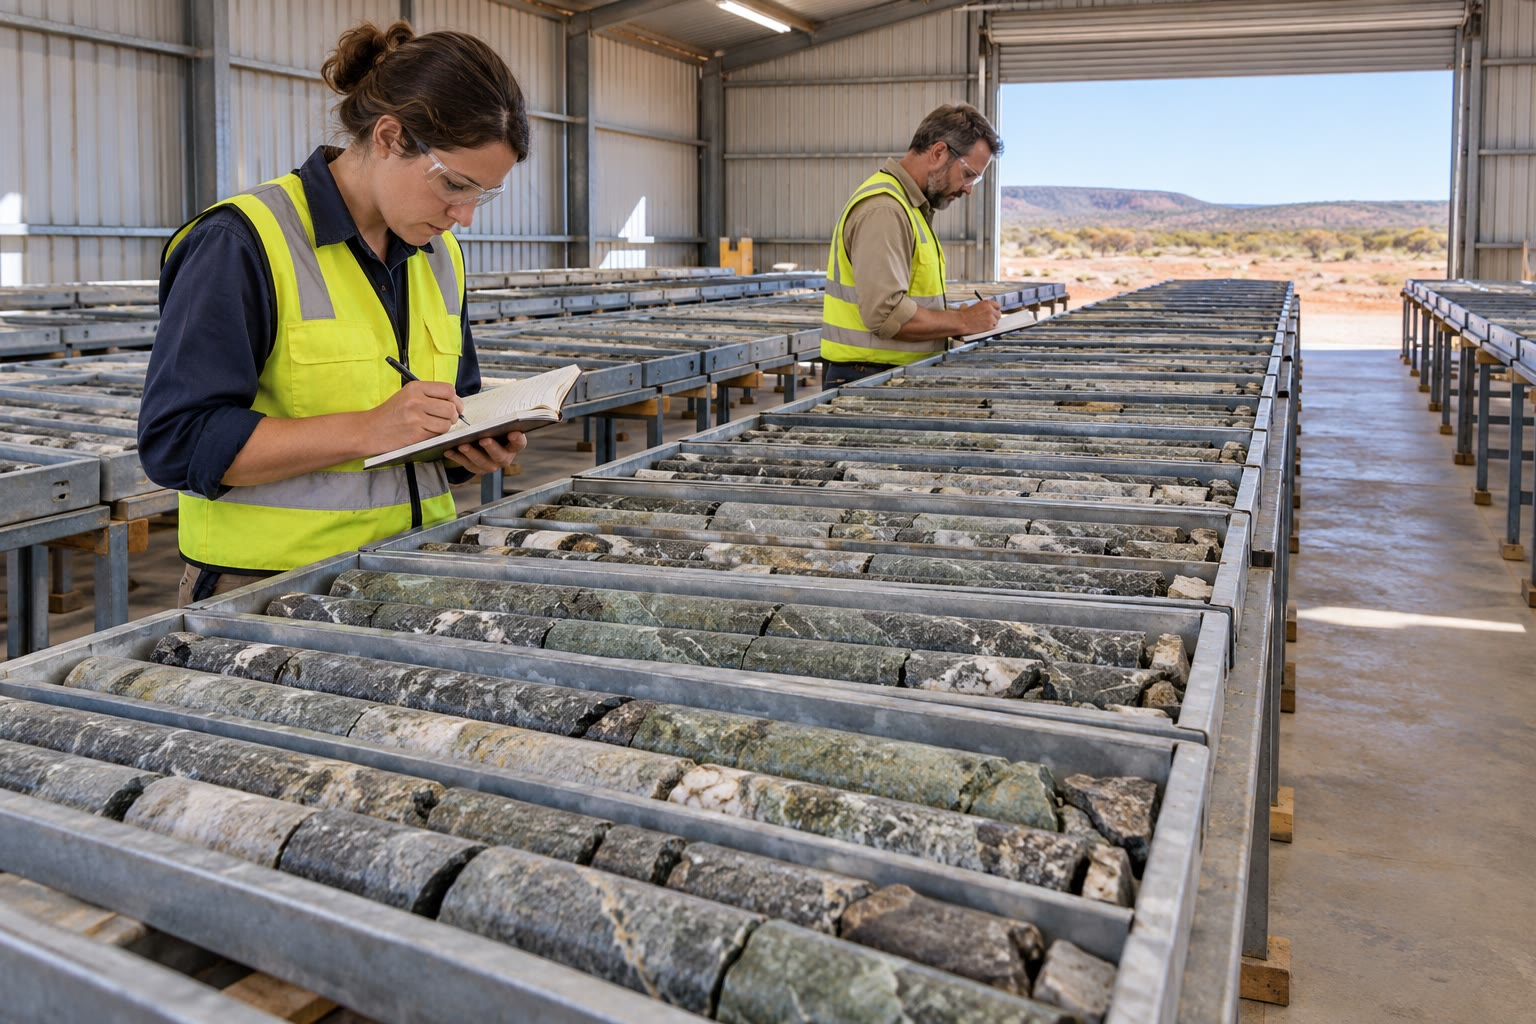
\includegraphics[width=0.56\linewidth]{images/book4/ai/b2-core-shed.jpg}
\par\smallskip{\small Gudang inti bor pada suatu proyek eksplorasi (ilustrasi buatan AI).}
\par\medskip\raggedright
Pada suatu proyek eksplorasi, inti dari setiap lubang bor dijajarkan di dalam baki logam menurut urutan
keluarnya dari tanah. Para ahli geologi menyusuri baki-baki itu, selang demi selang, dan mencatat batuan
apa itu, bagaimana alterasinya, urat mana yang memotongnya dan dalam proporsi berapa, serta sulfida apa yang
dimuatnya; mereka menandai tempat inti akan digergaji dan dicuplik. Deskripsi itu dibuat sebelum hasil analisis kadar dan
dibandingkan dengannya: zona alterasi atau tipe urat yang membawa logam menjadi hal yang
diikuti dari lubang ke lubang, dan dari deskripsi itu para ahli geologi menggambar penampang-penampang yang menjadi dasar perencanaan lubang
berikutnya.
\end{inthefield}

\section*{Latihan}\label{sec:b2:ore-deposits:exercises}

Data untuk latihan, kecuali dinyatakan lain: kerak benua atas, tembaga \qty{28}{ppm},
emas \qty{1.5}{ng/g}, kromium \qty{92}{ppm}; populasi tembaga porfiri pada
\cref{sec:b2:ore-deposits:grade-tonnage}, \omterm{def:b2:ore-deposits:grade}{tonase} $\log_{10}$ (Mt) dengan rata-rata 2.373 dan simpangan
baku 0.654, kadar $\log_{10}$ (\%) dengan rata-rata $-0.364$ dan simpangan baku 0.199, korelasi
$\rho = 0.100$. Bulatkan sampai tiga angka penting.
% ledger: rg03:ucc-trace, data:b4-porphyry-cu

\begin{exercise}[$\star$]\label{exo:b2:ore-deposits:1}
Tentukan \omterm{def:b2:ore-deposits:cf}{faktor konsentrasi} terhadap kerak atas dari: (a) bijih tembaga dengan
\qty{0.5}{\percent}; (b) bijih emas dengan \qty{6}{g/t}; (c) kromitit dengan \qty{90}{\percent}
kromit, dengan menganggap kromit sebagai FeCr$_2$O$_4$ (massa atom Cr 52.00, Fe 55.85, O 16.00).
\end{exercise}

\begin{exercise}[$\star$]\label{exo:b2:ore-deposits:2}
Batu Hijau dilaporkan sebesar \qty{914}{Mt} dengan \qty{0.53}{\percent} Cu dan \qty{0.40}{g/t} Au di atas
\omterm{def:b2:ore-deposits:grade}{kadar batas} \qty{0.3}{\percent}, dan sebesar \qty{1640}{Mt} dengan \qty{0.44}{\percent} Cu dan \qty{0.45}{g/t}
Au pada \omterm{def:b2:ore-deposits:grade}{kadar batas} terendah yang tersedia. (a) Tentukan tembaga (Mt) dan emas (t) yang terkandung pada setiap
perkiraan. (b) \omterm{def:b2:ore-deposits:grade}{Tonase} berapa dan tembaga berapa yang ditambahkan oleh blok-blok tambahan pada perkiraan kedua, dan dengan
kadar rata-rata berapa? (c) Mengapa kedua perkiraan itu benar?
\end{exercise}

\begin{exercise}[$\star$]\label{exo:b2:ore-deposits:3}
Dalam hukum Stokes kecepatan pengendapan butir berdiameter $d$ sebanding dengan $(\rho_s -
\rho_w)\,d^2$. Ambillah $\rho_w = 1.00$, kuarsa 2.65, emas 19.3, zirkon 4.7 (dalam
\unit{g.cm^{-3}}). (a) Berapa kali lebih cepat butir emas mengendap daripada butir kuarsa yang
berukuran sama? (b) Berapa perbandingan diameter butir emas dan butir kuarsa yang mengendap dengan
kecepatan yang sama? (c) Butir kuarsa mana yang mengendap seperti butir zirkon berukuran \qty{0.1}{mm}?
\end{exercise}

\begin{exercise}[$\star$]\label{exo:b2:ore-deposits:4}
Suatu bijih tembaga primer memiliki kadar \qty{0.4}{\percent}. Pelapukan melindi semua tembaganya sepanjang
ketebalan \qty{150}{m} dan mengendapkannya kembali dalam selimut setebal \qty{50}{m} tepat di bawahnya, dengan densitas
yang sama. (a) Tentukan kadar selimut itu. (b) Hal yang sama jika hanya \qty{80}{\percent} tembaga
yang terlindi diendapkan kembali. (c) Ketebalan terlindi berapa yang akan memberikan \qty{1.7}{\percent} dengan
pengendapan kembali yang lengkap?
\end{exercise}

\begin{exercise}[$\star\star$]\label{exo:b2:ore-deposits:5}
Suatu \omterm{def:b2:magma-emplacement:magma}{magma} memuat \qty{10}{ppb} platina dan \qty{200}{ppm} nikel; ambillah $D_{\mathrm{Pt}} =
10^4$ dan $D_{\mathrm{Ni}} = 500$. (a) Dengan memakai \eqref{eq:b2:ore-deposits:r-factor}, tentukan
kandungan platina (ppm) dan nikel (wt\%) dalam sulfida untuk $R = 100$, \num{1000}, \num{10000},
dan \num{100000}. (b) Tentukan limitnya untuk $R \to \infty$. (c) Jelaskan mengapa bijih nikel hanya
sedikit memberi tahu tentang $R$, sedangkan bijih platina banyak.
\end{exercise}

\begin{exercise}[$\star\star$]\label{exo:b2:ore-deposits:6}
Dengan memakai \eqref{eq:b2:ore-deposits:product} untuk populasi tembaga porfiri: (a) tentukan rata-rata dan
simpangan baku $\log_{10} M$, serta tembaga terkandung mediannya. (b) Berapa fraksi endapan yang
memuat lebih dari \qty{10}{Mt} tembaga? Berapa banyak dari 422? (c) Ulangi (b) dengan mengabaikan korelasi.
\end{exercise}

\begin{exercise}[$\star\star$]\label{exo:b2:ore-deposits:7}
Untuk endapan ilustratif dalam gambar ($T_0 = \qty{1000}{Mt}$, median \qty{0.40}{\percent},
$s = 0.60$), gunakan \eqref{eq:b2:ore-deposits:gt} untuk menentukan \omterm{def:b2:ore-deposits:grade}{tonase}, kadar rata-rata, dan tembaga terkandung
di atas \omterm{def:b2:ore-deposits:grade}{kadar batas} \qty{0.3}{\percent} dan \qty{0.6}{\percent}. Periksalah satu titik pada gambar.
\end{exercise}

\begin{exercise}[$\star\star$]\label{exo:b2:ore-deposits:8}
Suatu endapan porfiri memuat \qty{5}{Mt} tembaga. Misalkan fluida magmatiknya membawa \qty{1000}{ppm}
tembaga, yang separuhnya diendapkan dalam bijih, dan \omterm{def:b2:magma-emplacement:magma}{magma} itu melepaskan \qty{3.5}{\percent}
massanya sebagai fluida. (a) Tentukan massa fluida dan massa \omterm{def:b2:magma-emplacement:magma}{magma} yang diperlukan. (b) Tentukan volume
\omterm{def:b2:magma-emplacement:magma}{magma} itu, dengan densitas \qty{2600}{kg.m^{-3}}. (c) Jika \omterm{def:b2:magma-emplacement:magma}{magma} itu memuat \qty{50}{ppm} tembaga, berapa fraksi
tembaga itu yang berakhir di dalam bijih?
\end{exercise}

\begin{exercise}[$\star\star$]\label{exo:b2:ore-deposits:9}
Delapan sedimen sungai latar belakang memberikan $\log_{10}$ Cu (ppm) sebesar 1.30, 1.45, 1.38, 1.52, 1.41, 1.35,
1.48, dan 1.40. (a) Tentukan rata-rata dan simpangan baku (populasi) logaritma itu, median
latar belakang, dan ambang rata-rata ditambah dua simpangan baku, dalam ppm. (b) Suatu anak sungai
yang mengalirkan \qty{4}{km^2} tanah termineralisasi membawa sedimen dengan \qty{400}{ppm}; anak sungai itu bergabung dengan sungai yang
mengalirkan \qty{36}{km^2} dengan median latar belakang. Dengan menganggap setiap kilometer persegi menghasilkan
massa sedimen yang sama, apakah sedimen campurannya anomal? (c) Sampai luas daerah tangkapan total berapa
anomali itu tetap di atas ambang?
\end{exercise}

\begin{exercise}[$\star\star\star$]\label{exo:b2:ore-deposits:10}
(a) Buktikan $e^{su}\varphi(u) = e^{s^2/2}\varphi(u - s)$. (b) Turunkan rata-rata peubah
log-normal, $e^{\mu + s^2/2}$. (c) Tunjukkan bahwa fraksi logam di atas \omterm{def:b2:ore-deposits:grade}{kadar batas},
$\Phi(z + s)$, selalu melebihi fraksi \omterm{def:b2:ore-deposits:grade}{tonase}, $\Phi(z)$, lalu tafsirkan.
\end{exercise}

\begin{exercise}[$\star\star\star$]\label{exo:b2:ore-deposits:11}
(a) Dari \eqref{eq:b2:ore-deposits:r-factor}, tentukan $R$ saat $C_S$ mencapai fraksi $f$
dari batas atasnya $D\,C_L$. (b) Hitunglah untuk $f = 0.5$ dan $0.9$ dengan $D = 300$ (nikel) dan $D =
10^4$ (platina). (c) Bandingkan dengan rentang $R$ bijih nikel--tembaga dan terumbu PGE yang diberikan
dalam teks.
\end{exercise}

\begin{exercise}[$\star\star\star$]\label{exo:b2:ore-deposits:12}
(a) Untuk peubah log-normal $M$ dengan $\ln M$ bersimpangan baku $s$, tunjukkan bahwa endapan-endapan di atas
kuantil berorde $q$ memuat fraksi $\Phi\bigl(s - \Phi^{-1}(q)\bigr)$ dari logam total.
(b) Hitunglah untuk populasi porfiri dan $q = 0.9$. (c) Hal yang sama untuk $q = 0.99$; bandingkan dengan
keempat endapan terbesar, yang memuat \qty{26.6}{\percent} tembaga dalam kompilasi itu.
\end{exercise}
% ledger: data:b4-porphyry-cu

\begin{problem}[{Soal akhir pekan --- Suatu prospek porfiri}]\label{pb:b2:ore-deposits:1}
Suatu prospek porfiri (rekaan) telah dibor. Lubang penemuannya memotong delapan selang, dari atas
ke bawah (panjang dalam meter, kadar tembaga dalam persen): 30 m dengan 0.12; 40 dengan 0.35; 50 dengan 0.62; 60
dengan 0.48; 40 dengan 0.27; 30 dengan 0.81; 50 dengan 0.41; 30 dengan 0.18. Suatu studi geostatistik atas semua lubang
mendapati bahwa kadar blok berdistribusi log-normal, dengan median \qty{0.38}{\percent} dan $s = 0.55$ untuk
$\ln g$. Tubuh termineralisasi itu mendekati silinder vertikal berjari-jari \qty{450}{m} dan bertinggi
\qty{700}{m}, dengan densitas \qty{2.7}{t.m^{-3}}. Gunakan data latihan, dan bulatkan sampai tiga
angka penting (probabilitas sampai empat).

\noindent\textbf{Bagian I --- Lubang penemuan.}
\begin{enumerate}
  \item Tentukan panjang lubang yang dicuplik dan kadar rata-ratanya yang dibobot menurut panjang.
  \item Tentukan rata-rata aritmetika kedelapan kadar. Mengapa rata-rata berbobot adalah yang benar?
  \item Fraksi panjang mana yang di atas \qty{0.3}{\percent}, dan dengan kadar rata-rata berapa?
  \item Tentukan \omterm{def:b2:ore-deposits:cf}{faktor konsentrasi} kadar rata-rata berbobot terhadap kerak atas.
  \item Hal yang sama untuk selang terkaya.
  \item Tentukan kadar rata-rata semua blok endapan itu. Apakah lubang penemuan itu representatif?
\end{enumerate}

\noindent\textbf{Bagian II --- Tonase di atas kadar batas.}
\begin{enumerate}[resume]
  \item Tentukan volume dan \omterm{def:b2:ore-deposits:grade}{tonase} $T_0$ tubuh itu; pertahankan $T_0 = \qty{1200}{Mt}$.
  \item Untuk \omterm{def:b2:ore-deposits:grade}{kadar batas} \qty{0.3}{\percent}, tentukan $z$ dan fraksi blok yang di atasnya.
  \item Tentukan \omterm{def:b2:ore-deposits:grade}{tonase} di atas \omterm{def:b2:ore-deposits:grade}{kadar batas} 0.2, 0.3, dan \qty{0.5}{\percent}.
  \item Tentukan kadar rata-rata di atas \omterm{def:b2:ore-deposits:grade}{kadar batas} \qty{0.3}{\percent}.
  \item Hal yang sama di atas 0.2 dan \qty{0.5}{\percent}.
  \item Bila \omterm{def:b2:ore-deposits:grade}{kadar batas} dinaikkan dari 0.3 menjadi \qty{0.5}{\percent}: dengan faktor berapa \omterm{def:b2:ore-deposits:grade}{tonase} dan
        kadar rata-rata berubah?
  \item Pada \omterm{def:b2:ore-deposits:grade}{kadar batas} berapa separuh \omterm{def:b2:ore-deposits:grade}{tonase} dipertahankan, dan berapa kadar rata-ratanya?
\end{enumerate}

\noindent\textbf{Bagian III --- Prospek itu di antara porfiri-porfiri dunia.}
\begin{enumerate}[resume]
  \item Tentukan tembaga yang terkandung dalam seluruh tubuh, pada kadar rata-ratanya.
  \item Tentukan skor baku \omterm{def:b2:ore-deposits:grade}{tonasenya} dalam populasi dunia, dan persentilnya.
  \item Hal yang sama untuk kadar rata-ratanya.
  \item Tentukan simpangan baku $\log_{10} M$ dengan korelasi, dan tanpa korelasi.
  \item Tentukan persentil tembaga terkandungnya.
  \item Berapa banyak dari 422 endapan yang diharapkan memuat lebih banyak tembaga?
\end{enumerate}

\noindent\textbf{Bagian IV --- Tembaga di atas kadar batas.}
\begin{enumerate}[resume]
  \item Tentukan tembaga yang terkandung di atas \omterm{def:b2:ore-deposits:grade}{kadar batas} \qty{0.2}{\percent}.
  \item Hal yang sama di atas \qty{0.5}{\percent}.
  \item Berapa fraksi tembaga yang terletak di atas \qty{0.3}{\percent}, dan berapa fraksi
        \omterm{def:b2:ore-deposits:grade}{tonasenya}?
  \item Jelaskan mengapa menurunkan \omterm{def:b2:ore-deposits:grade}{kadar batas} di bawah \qty{0.3}{\percent} menambahkan banyak batuan dan sedikit
        tembaga, dengan memakai jawaban pertanyaan 9 dan 20.
  \item Sebagai ringkasan: berapa banyak tembaga yang dimuat prospek itu di atas \omterm{def:b2:ore-deposits:grade}{kadar batas} \qty{0.3}{\percent}?
\end{enumerate}
\end{problem}
